\documentclass{beamer}
\usepackage{xmpmulti}
\usepackage{caption}
\usepackage{subcaption}
\usepackage{epstopdf}
\usepackage{graphics}
\usepackage{tikz}
\usepackage{amsmath}
\usepackage{verbatim}
\usepackage{color}
\usepackage{natbib}
\usepackage{bibentry}
\bibliographystyle{apalike}
\usepackage{chngcntr}
\usepackage{color}
\usepackage[subnum]{cases}

\definecolor{links}{HTML}{2A1B81}
\hypersetup{colorlinks,linkcolor=blue,urlcolor=links}
\setbeamertemplate{navigation symbols}{}
\usepackage{caption}
\captionsetup[figure]{labelformat=empty}

\usetheme{Montpellier}
%\setbeameroption{show notes}
\beamersetuncovermixins{\opaqueness<1>{25}}{\opaqueness<2->{15}}

\date{\today}

\begin{document}


\title{Cognitive Ecology: System Complexity and Diversity of Models.}
%Here's how I can see your paper:
%A) motivation of big project: aggregation of diverse beliefs. Want to measure relationship of diverse beliefs to performance
%B) This paper: describing causal beliefs and measuring diversity
%C) In math, define a causal belief structure, and relate it to a probability density function
%D) In math, show how the Weitzman measure + the JS metric yield a measure of the diversity of probability density functions.
%E) In a simulation, describe 5 macroeconomic variables, create say 10 causal belief structures out of them.
%F) Specify the resulting probability density functions. Calculate diversity.
%G) Show that as you change how you create the 10 causal belief structures, the diversity measure changes in a plausible way.
%H)Conclude.



\author{Johannes Castner}
\institute{Columbia University}
\begin{frame}
\titlepage


\end{frame}

%\frame{\frametitle{Table of contents}\tableofcontents}

\begin{frame}
\frametitle{General Interest}
\begin{itemize}
\item Feedbacks between systems and beliefs 
\hfill \break
\item Complexity and Cognition
\hfill \break
\item Sustainable Development (Collective Intelligence and Collective Action) 
\end{itemize}
\end{frame}
\section{Overview}
\begin{frame}
\frametitle{Motivating example: Financial Bubbles}
 
Theories of Financial Bubbles \citep[optimists and pessimists, e.g][]{Scheinkman2003}: 

\begin{itemize}
\item are about institutions and beliefs: short-sale constraints in the presence of pessimists and optimists\\
\item pessimists sell all of their shares (exit the market)
\item optimists borrow and buy
\item the bubble ensues      
\item but they do not model where beliefs come from. \\
\end{itemize}

\vspace{0.5cm}

\begin{center}
My dissertation:\\
\end{center}
1) Shows that the complexity of the system and cognitive bounds jointly give rise to heterogeneity of beliefs; 2) builds an experimental platform to study belief dynamics; and 3) uses this platform to test the cognitive theory of financial bubbles.\\


\end{frame}

\section{Measuring Mental Models (Bayes Nets)}

\begin{frame}
\frametitle{Laboratory Experiments on System Complexity and Cognitive Diversity}
\small
\begin{figure}
A participant's goal (for example): predict Interest Rates. 
        \centering
        \begin{subfigure}[b]{0.5\textwidth}
                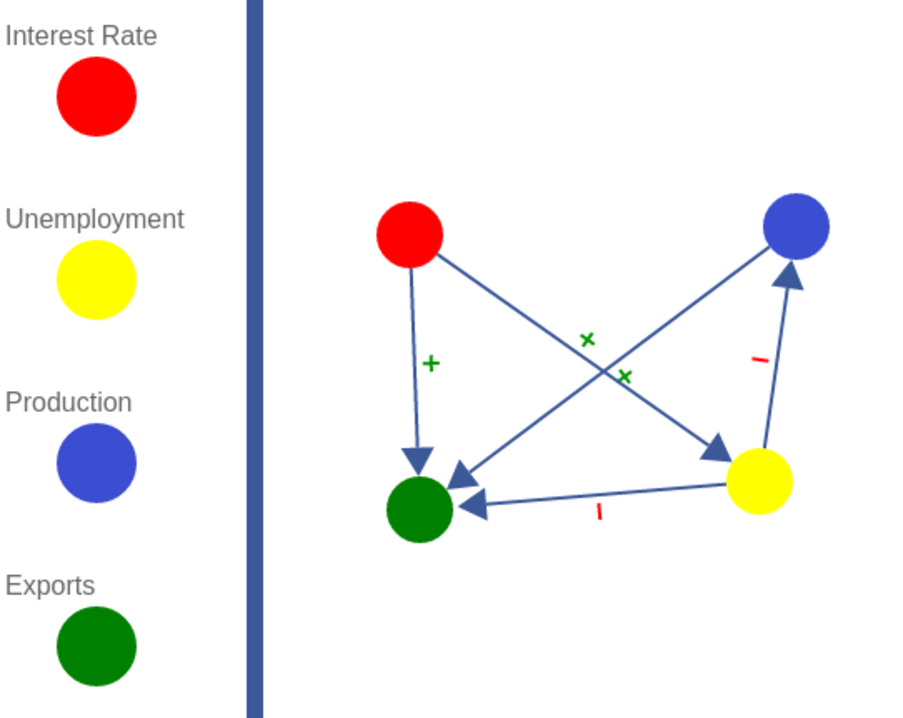
\includegraphics[width=\textwidth]{Complex.pdf}
                
        \end{subfigure}%
       \caption{A belief system about a financial system: The nodes are variables and the arrows are causal relations.}
\end{figure}

\end{frame}

\begin{frame}
\frametitle{Simple and Complex}
\begin{figure}
        \centering
       \begin{subfigure}{0.45\textwidth}
        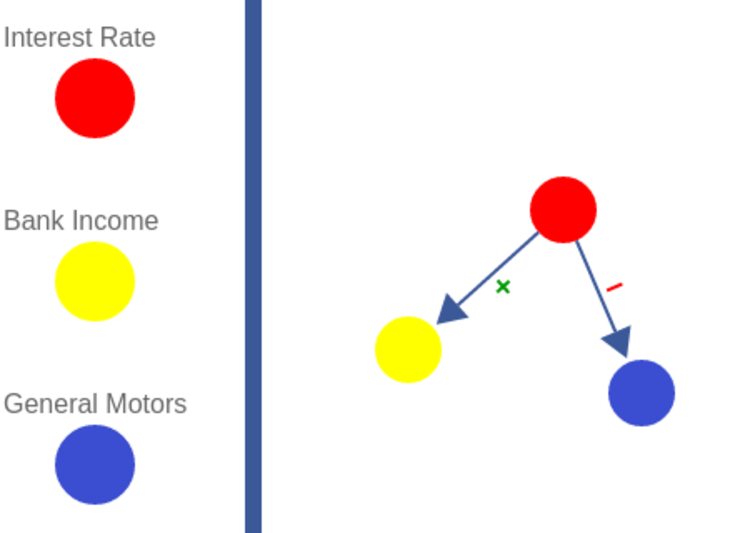
\includegraphics[width=\textwidth]{SimpleModel.pdf}
        
        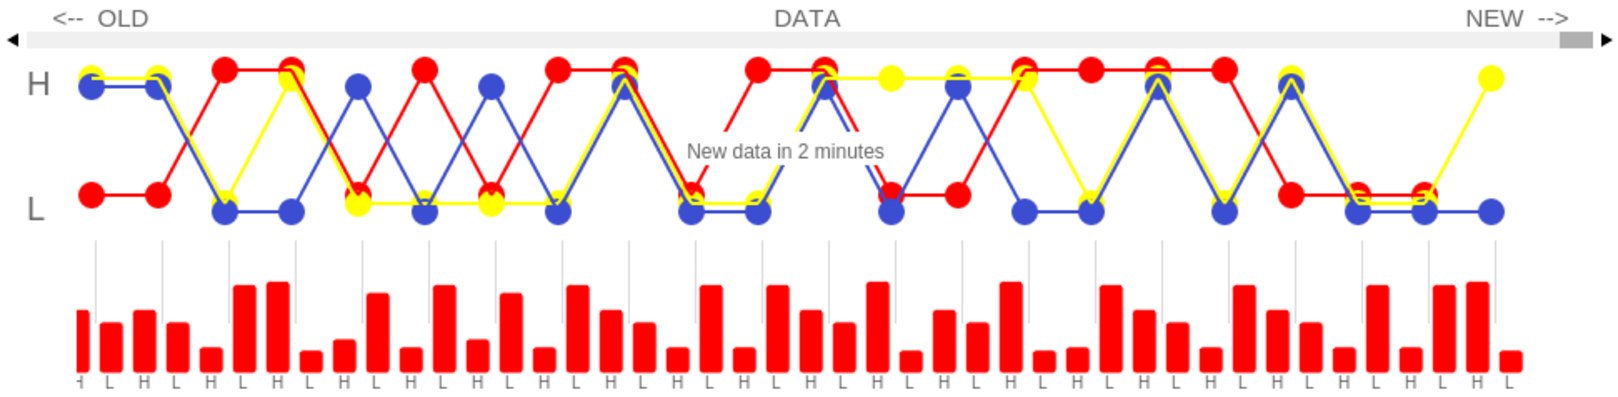
\includegraphics[width=\textwidth]{SimpleData.pdf}
                         \end{subfigure} \begin{subfigure}{0.45\textwidth}
        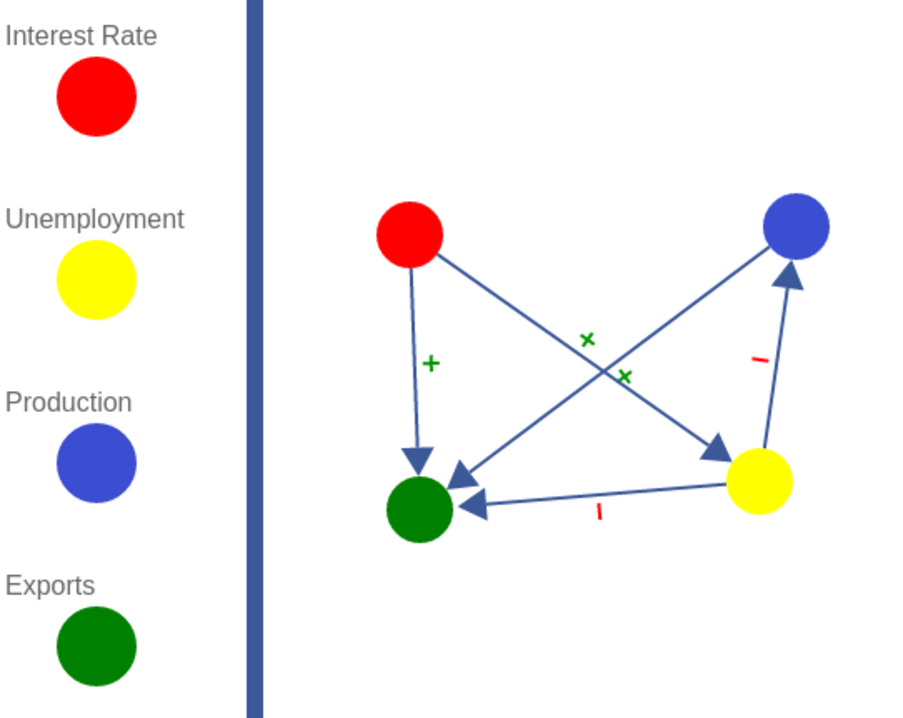
\includegraphics[width=0.9\textwidth]{Complex.pdf}
                %\caption{The Complex Case.}

         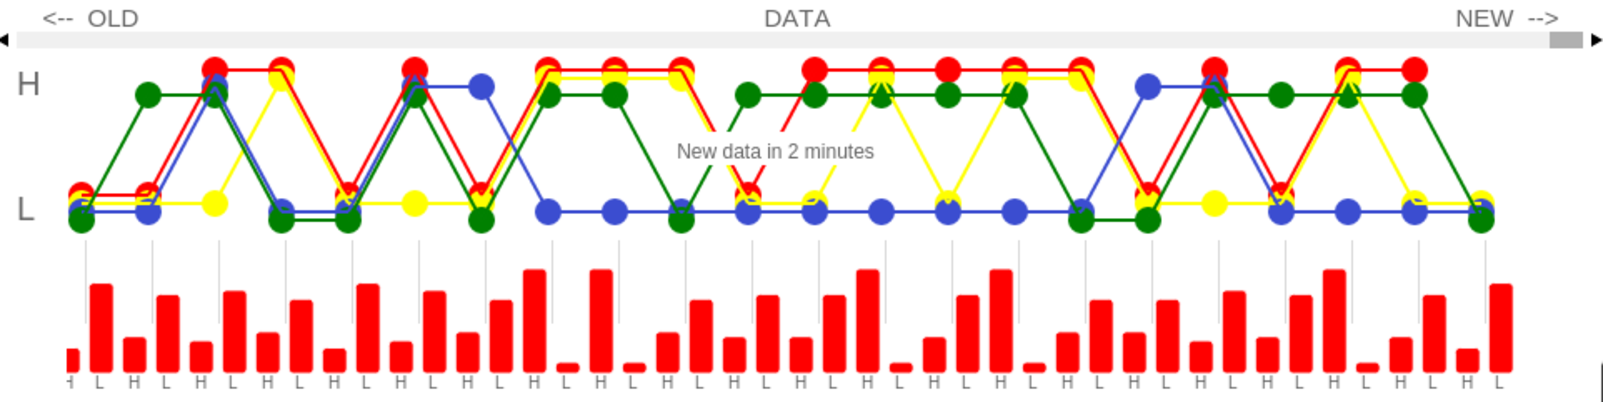
\includegraphics[width=\textwidth]{ComplexData.pdf}
        \end{subfigure}%
     
\end{figure}
\end{frame}
\section{Theory}
\begin{frame}
\frametitle{Measuring Cognitive Diversity}
\begin{definition}[$N$-Point Jensen-Shannon Divergence]
\begin{equation}
JSD(P_1, \ldots, P_N)= H\left(\sum_{i=1}^N\pi_iP_i\right)-\sum_{i=1}^N\pi_iH(P_i),
\end{equation}
\small
where $H(P)$ is the Shannon entropy for joint-distribution $P$. 
\end{definition} 
%This measures how much information on average one piece of data gives us (measured in bits) about the distribution it was drawn from, when it was drawn from one of the $N$ distributions, $P_i$, where the draw was done with uniform probability.
\begin{definition}[Cognitive Diversity]
Normalizing for group size I divide by $\sqrt{\log_2(N)}$ and I define Cognitive diversity as 
\begin{equation}
CD(P_1, \ldots, P_N)=\sqrt{\frac{JSD(P_1, \ldots, P_N)}{\log_2(N)}}.
\end{equation}
In the $2$ person case, this is a metric and I call the measure ``Cognitive Distance''. 
\end{definition} 
\normalsize 
\end{frame}

%\section{Sources of Diversity of Mental Models}
\begin{frame}
\frametitle{Sources of Diversity of Mental Models}
%All variables are binary $\left\{\text{H}, \text{L} \right\}$. 
\begin{enumerate}
\item Complexity of Causal Structure
\item Entropy 
\item Attention as a limited resource (Rational Inattention)
\end{enumerate}
\end{frame}

\begin{frame}
\frametitle{Complexity of Causal Structure}  
\begin{figure}
 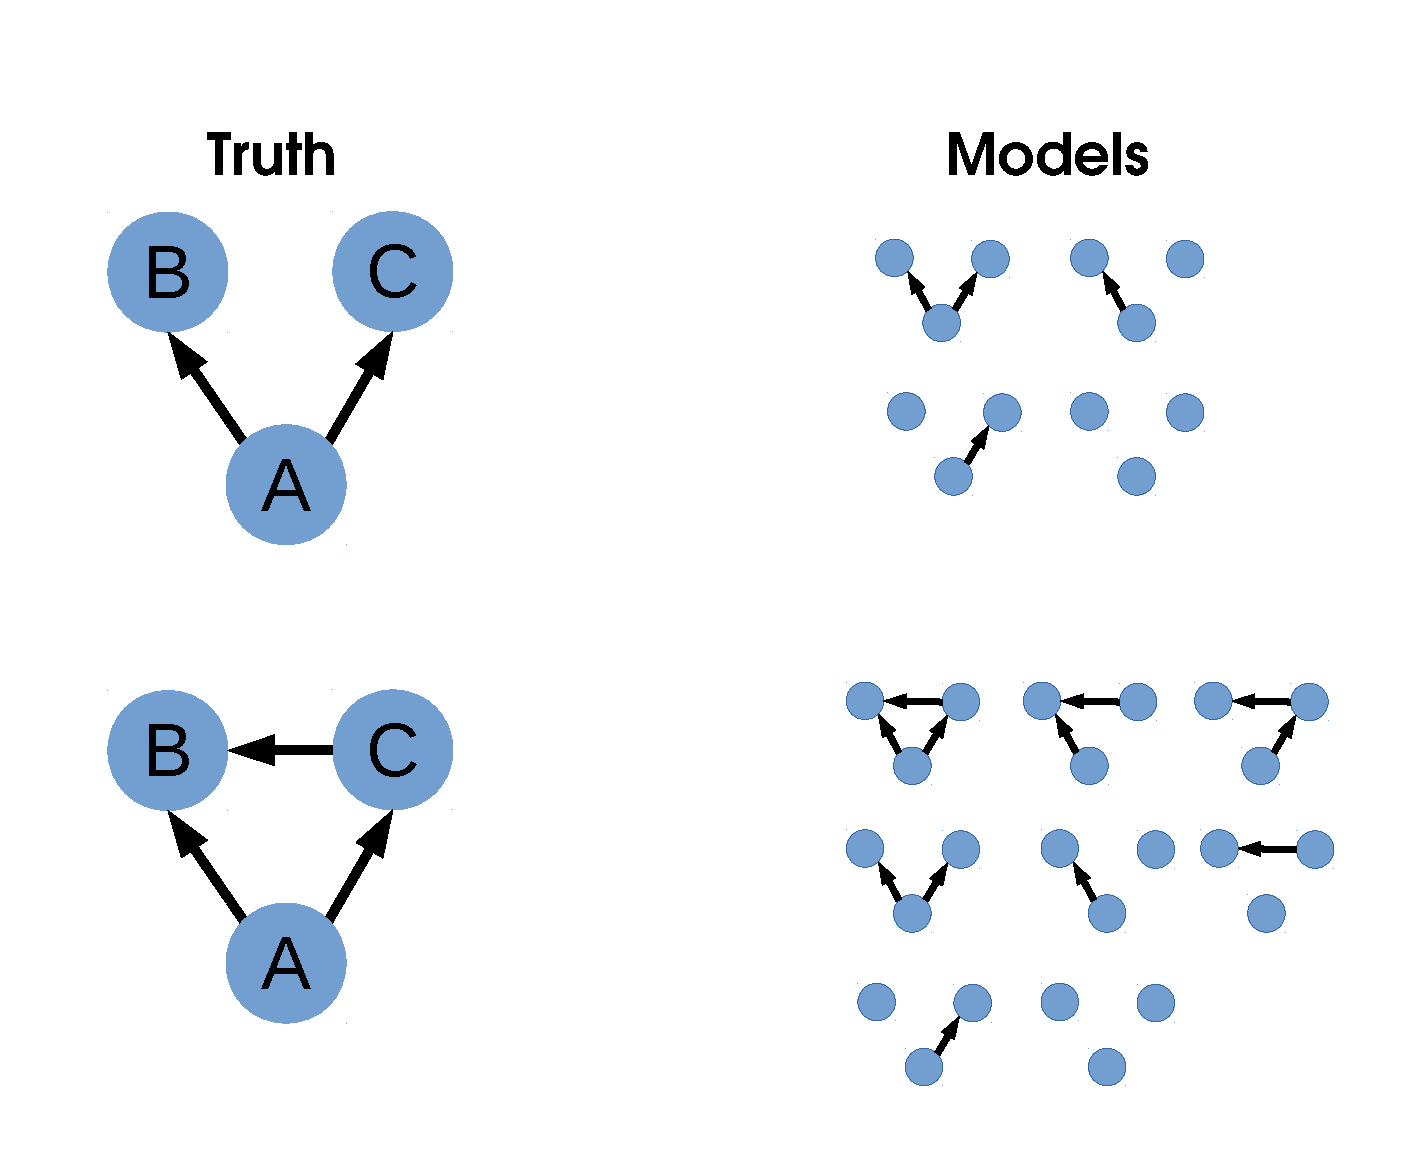
\includegraphics[width=0.5\textwidth]{TruthDiversity.pdf}
\end{figure}
There is a relation between the structural complexity of systems and the diversity of minds.
\end{frame}

\begin{frame}
\frametitle{Entropy}
If we think of causation as does \citet{Pearl88}, 
\begin{equation}
\small
\label{eq:noisy}
Pr(\text{Interest Rate}=1|\text{Unemployment}=a, Production=b)= 1-(1-\pi)^a(1-\pi)^b,
\end{equation}
\normalsize
where, $a$, $b$ $\in \left[0, 1\right]$ and where $1$ means high and $0$ means low, then 
\begin{itemize}
\item If $\pi=0$ there is no causation at all.
\item If $\pi=\frac{1}{2}$ entropy is maximal (the hardest case for inference).
\item If $\pi=1$ Equation \ref{eq:noisy} is the deterministic OR operator.
\end{itemize}
\end{frame}
\begin{frame}
\frametitle{Human Cognition as a Noisy Channel}
I use the Rational Inattention framework \citep{Woodford12} to show that
\begin{itemize} 
\item optimizing agents pay more attention to data points that are more frequent 
\item diversity of predictions arises in low probability states of systems through imprecise updating 
\end{itemize}
The more complex the system, the more low probability states it has and hence complexity induces diversity.   
\begin{figure}
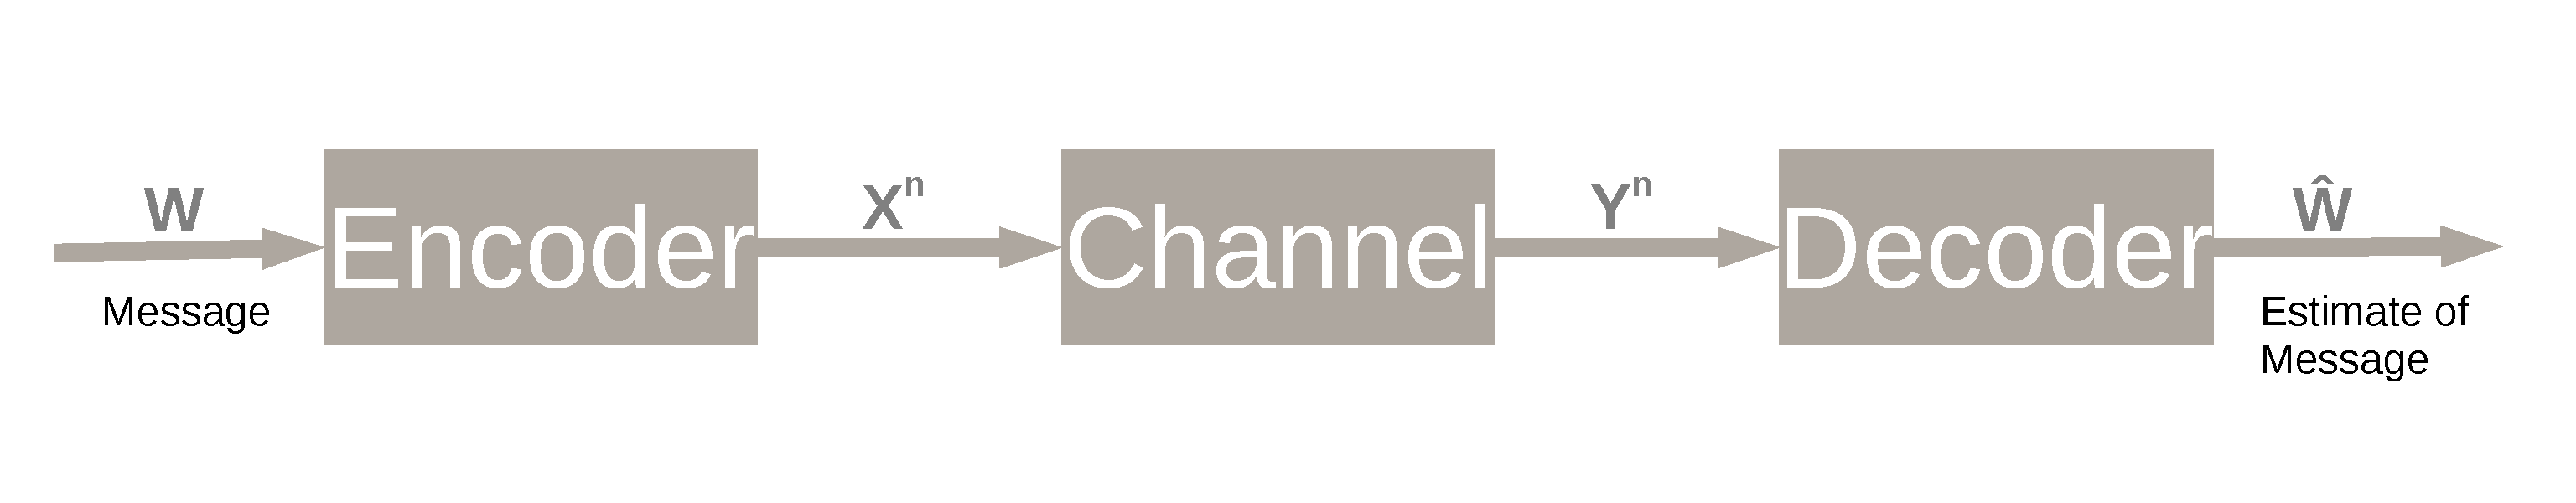
\includegraphics[width=\textwidth]{Channel.pdf}
\end{figure}

\end{frame}
\begin{frame}
\frametitle{The Near Future}
I will continue to triangulate 
\begin{itemize}
\item Information and Communication Theory
\item Experimental Social Science
\item Social Science Theory
\end{itemize}
extending my questions to
\begin{itemize}
\item Conformity of Beliefs
\item Political Manipulation of Beliefs
\item Cultural Norms and Social Aspects of Beliefs
\end{itemize}
\end{frame}
\bibliography{ResearchStatement}
\end{document}
